
\documentclass[../open-optimization/open-optimization.tex]{subfiles}

%%%%%%%%%
\begin{document}
%%%%%%%%%

\titlepic{
	\begin{center}
	\begin{tabular}{ccccc}
	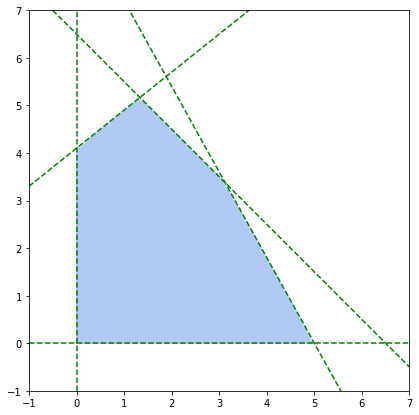
\includegraphics[scale = 0.3]{LP-feasible-region}  & \quad & 
	 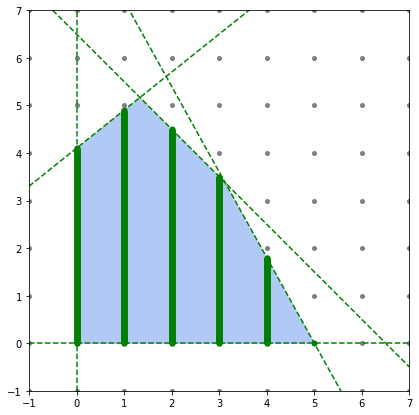
\includegraphics[scale = 0.3]{MIP-feasible-region} & \quad &
	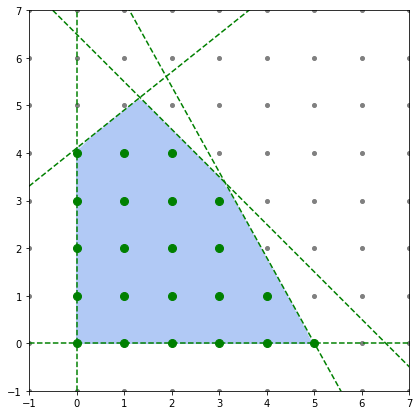
\includegraphics[scale = 0.3]{IP-feasible-region}%% \\
	%% LP && MIP && IP\\
	%% \\
	%% $Ax \leq b$ & &$Ax \leq b$ && $Ax \leq b$\\
	%% & &$x_1 \in \Z$ & &$x_1, x_2 \in \Z$
	\end{tabular}
	\end{center}\nopagebreak
        \begin{center}
          
\includegraphics[width=\linewidth]{../../../open-optimization-common/logos/logo-open-optimization-oer-wide}
        \end{center}
}
\maketitle
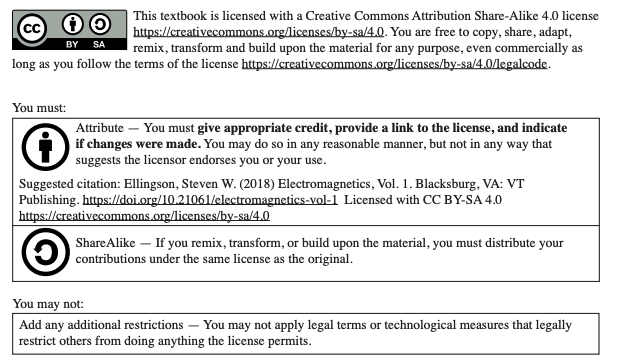
\includegraphics[scale = 0.65]{creative-commons-statement}


This work is done in alignment with the mission of UNESCO Open Educational Resources \url{https://en.unesco.org/themes/building-knowledge-societies/oer}
\begin{center}
\includegraphics[scale = 0.1]{Global_Open_Educational_Resources_Logo.svg}\footnotemark
\end{center}
\footnotetext{\url{https://en.wikipedia.org/wiki/Open_educational_resources\#/media/File:Global_Open_Educational_Resources_Logo.svg}}

The source code of this book is available from
\url{https://github.com/open-optimization/}

\newpage

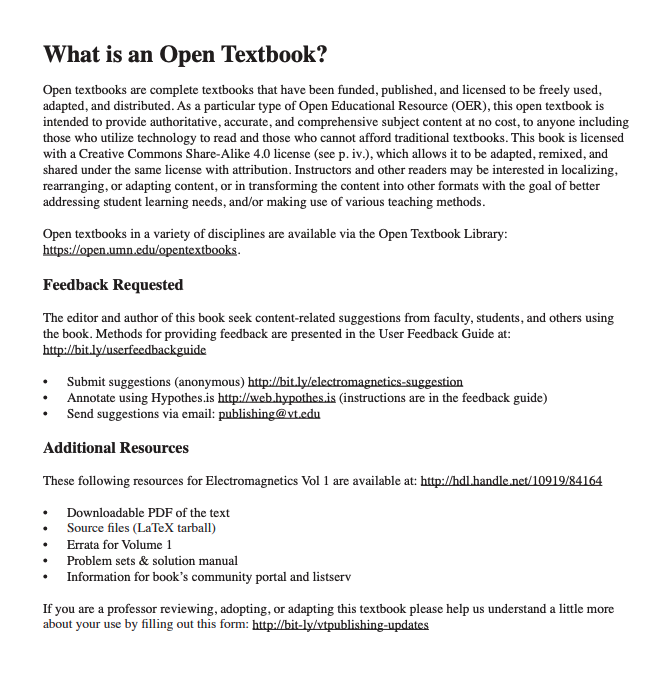
\includegraphics[scale = 0.65]{what-is-open-textbook}\footnotemark
\footnotetext{Take from open-source electromagnetics book}

\newpage

\section*{Preface}
%% FIXME: Move this preface text to .md and generate .tex from there.

Welcome to the Open Optimization - an ecosystem for open-source materials for teaching optimization and operations research.  This ecosystem is being formed to host open-source lecture notes, lecture slides, examples, code, figures, and textbooks on material and courses related to optimization.  All material will be licensed under Creative Commons Attribution-ShareAlike 4.0 International (CC BY-SA 4.0) that permits free reuse and alteration of the material provided the proper attribution is given.  All material posted will be not just open-source, but open-source code as well - including LaTeX, tikz, and other means of generating content.  This allows those interested in reusing material an easy way to change and adapt the material as needed.

Your contributions to this endeavor are greatly valued and appreciated.  You are being contacted directly due to the excellent material that you have on your website.  We hope you will help with this project and also use it as a resource for future courses, lectures, and presentations.

Content posted here may be adapted into freely available open-source textbooks published through ???.  All contributors to this repository will be acknowledged in any publication resulting from this material.  Please see ???? as an example.



\textbf{Goals:}
\begin{enumerate}
\item Create freely available content to make easier teaching, designing courses, writing presentations, and finding reusable content.
\item Create free textbooks for courses on optimization and operations research that are:
\begin{itemize}
\item Modern (up to date with current techniques and approaches)
\item Flexible (easy to adapt to the user?s choice of presentation of material)
\item Direct access to code examples (get students up and running faster)
\end{itemize}
\item Community collaboration on content authoring and revisions
\item Collect figures and images with source code for quality reproducibility
\item Host instructive code for optimization
\end{enumerate}










%%%%%%%%%
\end{document}
%%%%%%%%%
%%% Local Variables:
%%% mode: latex
%%% TeX-master: "../open-optimization/open-optimization"
%%% End:
